%% CS 2883R proposal, revised from the teammate's supplied first draft.
%% Original preserved verbatim in drafts/teammate-original.tex.
%% Revision: technical clarification, controls, prose, citations, adapted TikZ.
%% Sources inspected:
%% qqgjyx/overleaf_DriftNeRF @ 79946b56b0b951b03da3b58f4ea7062e4076bfa2
%% Q9gJYx/DriftNeRF @ e7fe12f260281e0748f42b5a70fb842be0bb8af2
%% arXiv:2610.29106v1, Sections 3.3--3.4 and Appendix D.
%% Build here: latexmk -pdf -interaction=nonstopmode main.tex
\documentclass[sigconf,nonacm]{acmart}
\setcopyright{none}
\settopmatter{printacmref=false,printfolios=true}
\usepackage{tikz}
\usetikzlibrary{arrows.meta,calc,positioning}
\usepackage{graphicx}
\usepackage[capitalise,noabbrev]{cleveref}
% Notation used in the proposal and adapted schematic.
\newcommand{\vx}{\boldsymbol{x}}
\newcommand{\sg}{\operatorname{sg}}


\begin{document}
\title{Sampling Dependence in DriftNeRF's Density Consensus}
\subtitle{CS 2883R: Final Project Proposal, Fall 2026}
\author{Juntang Wang}
\affiliation{\institution{Harvard University}\city{Cambridge}\country{USA}}
\email{juntangwang@g.harvard.edu}
\author{Ciro Zhang}
\affiliation{\institution{Harvard University}\city{Cambridge}\country{USA}}
\email{cirozhang@g.harvard.edu}
\renewcommand{\shortauthors}{Wang and Zhang}
% Adapted from DriftNeRF's images/fig-overview.tex: ray/sample geometry,
% contrasting anchor/candidate colors, proximity links, rounded consensus box.
% https://github.com/qqgjyx/overleaf_DriftNeRF/blob/79946b56b0b951b03da3b58f4ea7062e4076bfa2/images/fig-overview.tex
% Citation: Wang et al., arXiv:2610.29106v1 (CC BY 4.0).
% Changes: compact two-panel layout, input-ray labels, equal candidate counts,
% stratified off-ray queries, explicit detached targets. No result data.
% Blank lines are commented because acmart collects teaser content as an argument.
\begin{teaserfigure}
\centering
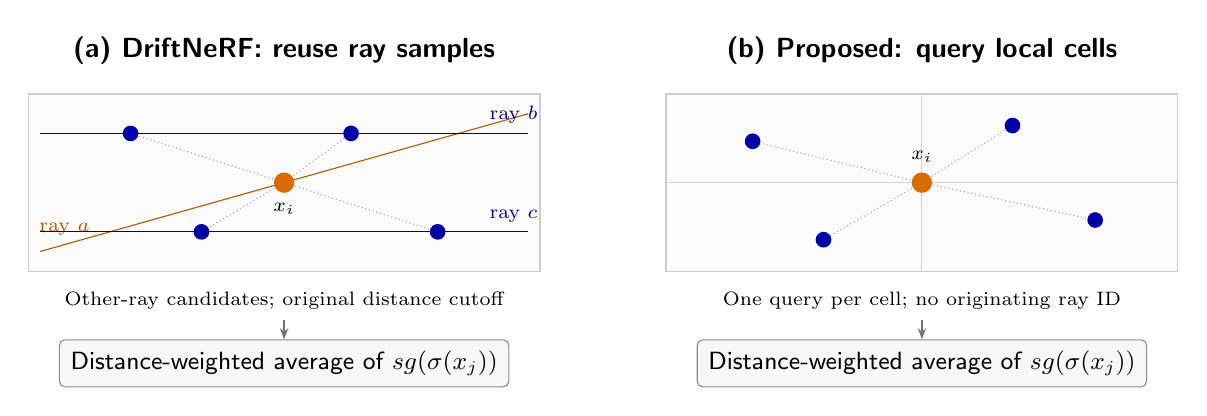
\begin{tikzpicture}[
  x=1cm,y=1cm,font=\sffamily\small,
  candidate/.style={circle,fill=blue!65!black,inner sep=2pt},
  anchorpoint/.style={circle,fill=orange!85!black,inner sep=2.6pt},
  arr/.style={-{Stealth[length=4pt]},semithick},
  target/.style={draw=black!45,rounded corners=2pt,fill=black!3,
    minimum height=0.55cm,align=center,inner sep=4pt}
]
\begin{scope}
  \node[font=\sffamily\bfseries] at (3.45,2.8)
    {(a) DriftNeRF: reuse ray samples};
  \draw[gray!40,fill=gray!3] (0.2,0) rectangle (6.7,2.25);
  \draw[orange!70!black,thin] (0.35,0.25) -- (6.55,2.0)
    node[pos=0.05,above,font=\scriptsize] {ray $a$};
  \draw[blue!55!black,thin] (0.35,1.75) -- (6.55,1.75)
    node[pos=0.97,above,font=\scriptsize] {ray $b$};
  \draw[blue!55!black,thin] (0.35,0.5) -- (6.55,0.5)
    node[pos=0.97,above,font=\scriptsize] {ray $c$};
  \coordinate (a) at (3.45,1.125);
  \foreach \x/\y in {1.5/1.75,4.3/1.75,2.4/0.5,5.4/0.5}{
    \draw[black!35,densely dotted] (a) -- (\x,\y);
    \node[candidate] at (\x,\y) {};
  }
  \node[anchorpoint,label={[font=\scriptsize]below:$\vx_i$}] at (a) {};
  \node[font=\scriptsize,align=center] at (3.45,-0.38)
    {Other-ray candidates; original distance cutoff};
  \node[target] (leftTarget) at (3.45,-1.17)
    {Distance-weighted average of $\sg(\sigma(\vx_j))$};
  \draw[arr,black!55] (3.45,-0.62) -- (leftTarget.north);
\end{scope}
\begin{scope}[xshift=8.1cm]
  \node[font=\sffamily\bfseries] at (3.45,2.8)
    {(b) Proposed: query local cells};
  \draw[gray!40,fill=gray!3] (0.2,0) rectangle (6.7,2.25);
  \draw[gray!35] (3.45,0) -- (3.45,2.25);
  \draw[gray!35] (0.2,1.125) -- (6.7,1.125);
  \coordinate (a) at (3.45,1.125);
  \foreach \x/\y in {1.3/1.65,4.6/1.85,2.2/0.4,5.65/0.65}{
    \draw[black!35,densely dotted] (a) -- (\x,\y);
    \node[candidate] at (\x,\y) {};
  }
  \node[anchorpoint,label={[font=\scriptsize]above:$\vx_i$}] at (a) {};
  \node[font=\scriptsize,align=center] at (3.45,-0.38)
    {One query per cell; no originating ray ID};
  \node[target] (rightTarget) at (3.45,-1.17)
    {Distance-weighted average of $\sg(\sigma(\vx_j))$};
  \draw[arr,black!55] (3.45,-0.62) -- (rightTarget.north);
\end{scope}
\end{tikzpicture}
\caption{Comparison of sampling strategies, adapted from DriftNeRF~\citep{wang2026driftnerf}. DriftNeRF reuses nearby samples from other camera rays, while our proposed approach queries one point in each local cell. Both form a distance-weighted target from the candidate densities. Orange marks the anchor and blue marks the candidates.}
\label{fig:sampling-hypothesis}
\Description{Left: four candidates lie on other camera rays. Right: four candidates are spread across local cells. Dotted lines connect each candidate to the anchor.}
\end{teaserfigure}

\maketitle
\raggedbottom
\balance

%% =================================================================
%% Research goal and problem statement
%% =================================================================
\section{Research goal and problem statement}\label{sec:goal}

Reconstructing a 3D scene from only a few images is challenging because different geometric configurations can reproduce the same observed views. Consequently, a Neural Radiance Field (NeRF)~\citep{mildenhall2020nerf} may fit its training images while still producing floating artifacts or incorrect geometry when task to rendered from new viewpoints. Thus, photometric reconstruction loss alone does not sufficiently constrain scene geometry, as an incorrect configuration can still reproduce the observed images. Improving reconstruction under limited observations is important for applications where capturing dense image collections is impractical.

DriftNeRF ~\citep{wang2026driftnerf}  addresses this problem by encouraging the model to predict similar densities at nearby points sampled along different camera rays. For each point, it computes a target density by averaging neighboring predictions, giving more weight to closer points. However, the candidate points are still drawn from the renderer's existing samples, whose spatial distribution depends on camera coverage and ray sampling. Thus, uniform selection from this pool does not necessary imply the uniform coverage of the underlying 3D neighborhood. Regions containing more samples can therefore contribute more strongly to the consensus target.

This raises an open research question: how much does density consensus reflect the actual reconstructed geometry, and how much does it depend on where samples are concentrated? We hypothesize that this dependence can sometimes reinforce incorrect density estimates as shown in \cref{fig:sampling-hypothesis}. For example, concentrating samples around an incorrectly reconstructed density peak could increase that region's influence on nearby targets. However, surface-focused sampling may also provide useful guidance by emphasizing genuine structures. The effect of balancing these contributions must therefore be investigated empirically.

This project will study how sample placement affects density consensus and test an alternative that uses more evenly distributed points within each local neighborhood. The main challenges we foresee are separating sampling effects from changes in the learned geometry, preserving thin structures, and keeping the extra computation manageable. We will use a small subset of NeRF-Synthetic, focusing on static scenes with known camera poses and only a few input views. Our goal is to determine when balanced sampling makes consensus targets less sensitive to sample placement and whether this leads to better reconstruction from new viewpoints.


%% =================================================================
%% Relationship to prior work
%% =================================================================
\section{Relationship to prior work}\label{sec:related}

Many existing works on sparse-view NeRF introduce additional constraints to reduce overfitting and improve novel-view synthesis. For example, FreeNeRF~\citep{yang2023freenerf} progressively exposes positional-encoding frequencies during training and penalizes density near cameras. RegNeRF~\citep{niemeyer2022regnerf} regularizes geometry and appearance in patches rendered from unobserved viewpoints and gradually expands its sampling space. These approaches motivate examining how regularization and sampling interact under limited observations.

Our project builds directly on DriftNeRF~\citep{wang2026driftnerf}, coauthored by Juntang Wang. We retain its field representation, detached-target update, and warmup schedule. The proposed extension changes how candidate points are obtained for the density average. We will compare renderer-derived candidates with independent uniform local queries and stratified local queries. This comparison distinguishes the effect of introducing off-ray queries from the additional effect of spatial stratification.

%% =================================================================
%% Proposed investigation
%% =================================================================
\clearpage
\section{Proposed method}

\paragraph{Testing the effect of sampling.}
We will first freeze a trained NeRF and fix a set of anchor points and the renderer sample pool. Repeated draws from that pool will show how much the original consensus targets vary. We will also construct targets using independent uniform and stratified local queries, repeating each scheme at a fixed query budget. We will compare target means, variability, and the direction and magnitude of the suggested density corrections. For the original method, we will record how often anchors have eligible neighbors. These diagnostics describe the training signal; lower variability alone does not establish better geometry.

\paragraph{Balanced neighborhood sampling.}
We propose dividing a cube centered on each anchor into equal-volume cells and sampling one point uniformly within each cell. The cube will be small enough that all its points lie within the original distance cutoff. The same NeRF will predict densities at these locations. We will combine them using the original exponential distance weighting and treat the resulting average as a fixed target during each update.

Unlike the original candidates, these new points have no originating camera-ray identifiers. Their eligibility is spatial, so this extension changes cross-ray consensus into a local field regularizer. It requires additional density evaluations, but no additional images or depth supervision. Anchor selection will remain unchanged.

\paragraph{Controls.}
The primary control will sample independent uniform points in the same cube. In the frozen-field analysis, the two off-ray schemes will use identical fields, anchors, neighborhoods, distance kernels, and numbers of queries per anchor. This isolates the effect of stratification. Comparison with original DriftNeRF also changes the spatial support and ray-eligibility rule, so it measures the combined effect of those changes.

\paragraph{Training.}
Each regularized variant will retain the image reconstruction loss and add a penalty for differences between anchor density and its detached target:
\begin{equation}
\mathcal{L}=\mathcal{L}_{\mathrm{render}}
+\lambda(t)\frac{1}{|\mathcal{A}|}
\sum_{i\in\mathcal{A}}
\bigl(\sigma_{\theta}(\mathbf{x}_i)-\mathrm{sg}(\mu_i)\bigr)^2.
\end{equation}
Here $\mathcal{A}$ contains valid anchors, $\mu_i$ is the distance-weighted neighborhood average, and $\mathrm{sg}$ denotes stop-gradient. Anchors without eligible candidates are excluded, and the auxiliary term is skipped if none are valid. As in DriftNeRF, the penalty weight rises linearly over the first 10\% of training. We will use a shared penalty weight for the primary comparison and examine a few neighborhood sizes, query counts, and penalty strengths as sensitivity checks.

\paragraph{Evaluation.}
We will compare vanilla NeRF, original DriftNeRF, independent uniform local queries, and stratified local queries using matched input views, initialization seeds, architectures, and training steps. We will report PSNR, SSIM, and LPIPS on held-out views, summarize variation across matched seeds, and inspect floaters and thin structures. Test views will be reserved for final evaluation rather than parameter selection.

We will also report elapsed training time and total density-query counts. DriftNeRF reuses a candidate pool shared across anchors, whereas the extension makes new queries for each anchor; equal candidate counts therefore do not imply equal computation. The extension will be useful if repeatable quality gains justify its computational cost while preserving thin structures. A reduction in target variability without improved rendering would instead identify a limitation of the proposed approach.

%% =================================================================
%% AI usage acknowledgement
%% =================================================================
\section*{AI usage acknowledgement}\label{sec:ai}
OpenAI Codex was used for brainstorming and minor technical feedback, and the TikZ schematic draft. No experiments were run for this proposal.
% AUTHOR REVIEW: Update this acknowledgement after your own final rewrite to
% reflect actual use. Add any other AI tool used for the first draft/schematic.
% AUTHOR REVIEW: Confirm individual contributions before the final report.

\bibliographystyle{ACM-Reference-Format}
\bibliography{ref}
\end{document}
